\documentclass[a4paper, 12pt]{article}

\usepackage{amsmath}
\usepackage{amssymb}
\usepackage{graphicx}
\usepackage{xspace}
\usepackage{cleveref}
\usepackage{booktabs}
\usepackage[parfill]{parskip}
\usepackage{booktabs}


\newcommand{\pt}{\ensuremath{p_{\mathrm{T}}}\xspace}

\begin{document}

\section{Introduction}
Herein lines some documentation on the HitFinder module in Delphes, and how I made it. 

This HitFinder module repeats the algorithm found within the ParticlePropagator module, except N times, where N is the number of ``surfaces''. 
The surfaces correspond to barrel layers, or end-cap layers (in this module, they simply correspond to two-dimensional surfaces, there are no modules or services). 
One can apply a pT cut to the input particles, as, for example, low momentum particle would not reach certain regions of the detector. 

Within Delphes, I added a Hit class that contains the 4-position of each particle hit, and the reference to the Delphes particle. 

\section{From hits to tracks}
The distribution of vertices from a sample of 100 events (overlaid with a mean pileup of 200) is shown in \ref{fig:vertices}.
The width of the distribution is $\sigma = 53$\,mm 
\begin{figure}
  \centering
  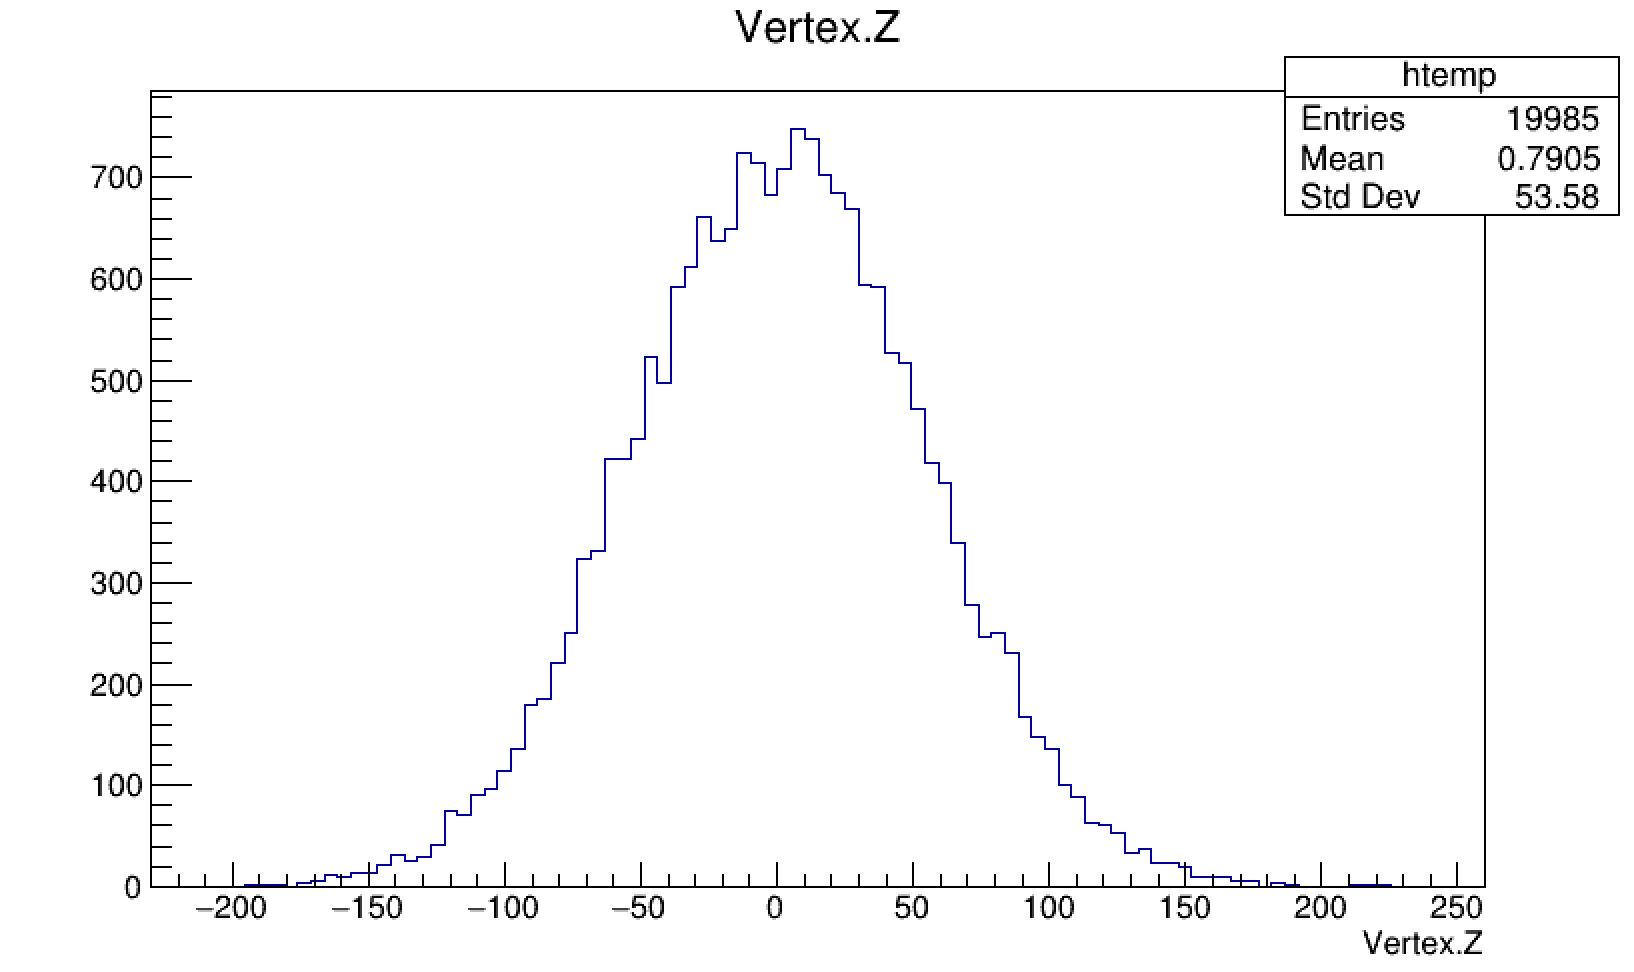
\includegraphics[width=0.5\linewidth]{images/vertexDistribution}
  \caption{Distribution of vertices in 100 ttbar events (with mean pileup 200) and 100 TeV.}
  \label{fig:vertices}
\end{figure}

\subsection{The basic tracking}
\subsubsection{From outside to in}
For the basic tracking algorithm, a coincidence of three tracks is required, starting from a hit in the outer layer, and falling within a cone of $3\sigma$ around the detector coordinate origin. 

\begin{figure}
  \centering
  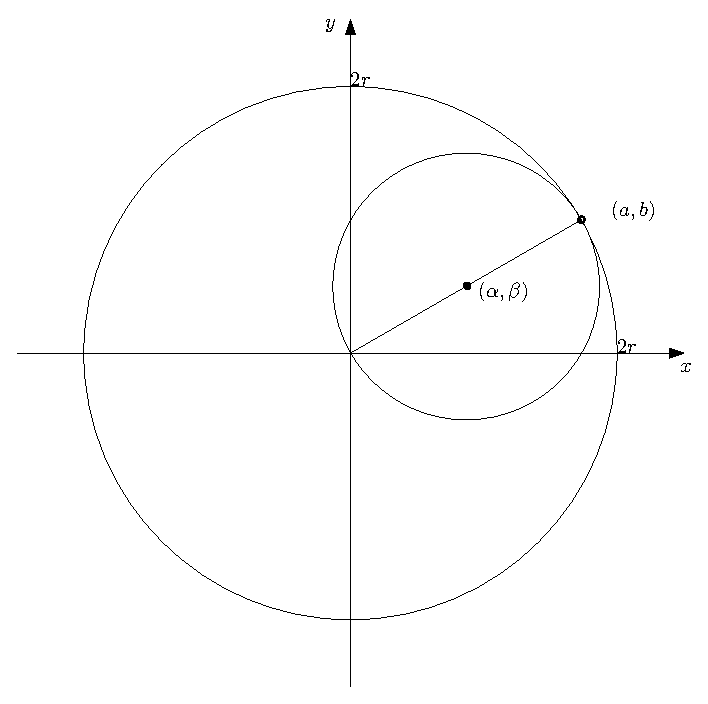
\includegraphics[width=0.5\linewidth]{images/geometry1}
  \caption{}
  \label{fig:circles1}
\end{figure}

Given a point $p= (a, b)$ on a circle of radius $2r$, the midpoint of the line from the origin to $p$ has the coordinates $(\alpha, \beta) = (a/2, b/2)$. 
Therefore, the equation of the smaller circle shown in \cref{fig:circles1} is
\begin{equation}
  \Big( x - \frac{a}{2} \Big)^2 + \Big( y - \frac{b}{2} \Big)^2 = r^2.
\end{equation}
We are actually interested in the intersection of the small circle in \cref{fig:circles1} with another circle, centered on the origin as displayed in \cref{fig:circles2}. 
Using the notation of the \cref{fig:circles2} we must combine
\begin{equation}
  x^2 + y^2 = r_2^2 \quad \mathrm{and} \quad (x - \alpha)^2 + (y - \beta)^2 = r^2,
  \label{eq:toSolve1}
\end{equation}
where for notational simplicity we have used $r = r_1 / 2$. 
Eliminating $y$ \cref{eq:toSolve1} gives
\begin{align}
  \Big( x - \alpha \Big)^2 + \Big( \sqrt{r_2^2 - x^2} - \beta \Big)^2 = & ~ r^2 \\
  x^2 + \alpha^2 - 2x\alpha + r_2^2 - x^2 + \beta^2 -2\beta \sqrt{r_2^2 - x^2} = & ~ r^2 \\
  (\alpha ^2 + \beta^2) -2 x \alpha +r_2^2 -2\beta\sqrt{r_2^2 - x^2} = & ~ r^2.  
\end{align}
Using $\alpha^2 + \beta^2 = r^2$,
\begin{align}
  r_2 ^2 & = 2x\alpha + 2\beta \sqrt{r_2^2 - x^2} \\
  (r_2^2 - 2\alpha x )^2 & = 4\beta^2 (r_2^2 - x^2) \\
  r_2^4  + 4\alpha^2 x^2 - 4r_2^2 \alpha x & = 4\beta^2 (r_2^2 - x^2) \\
  4x^2 (\alpha^2 + \beta^2) - 4r_2^2 \alpha x + r_2^4 -4\beta^2 r_2^2 & = 0.
\end{align}
Again using $\alpha^2 + \beta^2 = r^2$ leaves us with the quadratic
\begin{equation}
  4r^2 x^2 -4 r_2^2 \alpha x +r_2^2(r_2^2 -4 \beta^2) = 0
\end{equation}
and therefore, 
\begin{equation}
  x  = \frac{r_2^2 \alpha \pm \sqrt{r_2^4\alpha^2 - r^2 r_2^2(r_2^2 - 4\beta^2)}}{2r^2}.
\end{equation}
In the case that $\beta = 0$, then $r=\alpha$ and the above simplifies to $x = \frac{r_2^2}{2r}$.
Likewise for $y$ we find
\begin{equation}
  y  = \frac{r_2^2 \beta \pm \sqrt{r_2^4\beta^2 - r^2 r_2^2(r_2^2 - 4\alpha^2)}}{2r^2},
\end{equation}
which in the case $\alpha = 0$ simplifies to $y = \frac{r_2^2}{2r}$ (with $r=\beta$).

\begin{figure}
  \centering
  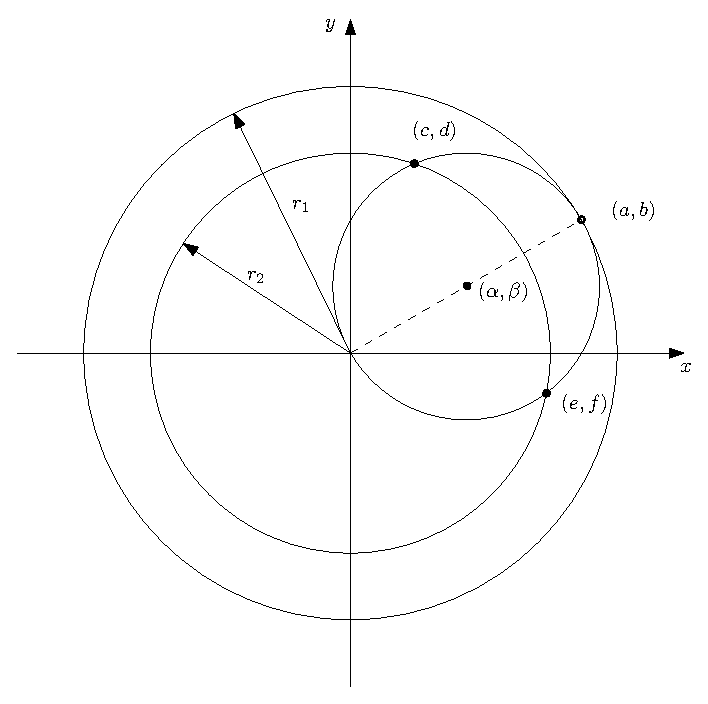
\includegraphics[width=0.5\linewidth]{images/geometry2.eps}
  \caption{}
  \label{fig:circles2}
\end{figure}

\subsubsection{From inside to out}
This second algorithm is used to create tracks starting from a hit in the innermost layer, 
and then finding matching hits in the outer layers. 
In the $r$--$z$ plane, two lines are drawn from the hit location to the edges of the luminous region along the beamline, these lines are extended outwards, and any hit within the two lines are matched
to the inner hit. 

\begin{figure}
  \centering
  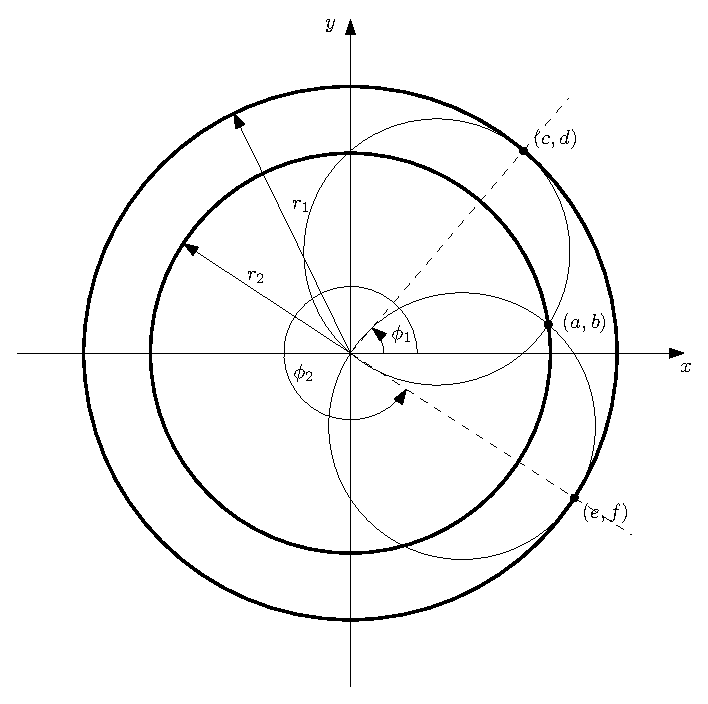
\includegraphics[width=0.5\linewidth]{images/geometry3.eps}
  \caption{}
  \label{fig:circles3}
\end{figure}

In the $r$--$\phi$ plane it is considered that the hit can traverse to the outermost layer in a circle.
Given that the charge of the particle is not known, the trajectory can curve in one of two directions.
We wish to find limits in $\phi$ to which the particle hits can be matched. 
With respect to \cref{fig:circles3} the algorithm proceeds as follows:
\begin{itemize}
  \item A hit is found in the innermost layer (which has radius $r_2$) at point $(a, b)$. 
  \item In the extreme case, the particle would bend in a circle in one direction or another, and so would end up at either point $p_1 = (c, d)$ or point $p_2 = (e, f)$. 
  \item A hit is matched if any hit in the outer layers lie within $\phi_1$ and $\phi_2$. 
  \item The angle between any $p_1$ and $p_2$ will always been the same, and so this only needs to be calculated once per geometry.  
\end{itemize}
Setting the problem up, we want to find the equations of the circles intersecting the origin and point $(a, b)$, i.e. solve
\begin{equation}
  (x - \alpha)^2 + (y - \beta)^2 = (r_1/2)^2, \quad a \in {x}, b \in {y} 
  \label{eq:circInToOut1}
\end{equation}
This amounts to finding the centre of these circles, the coordinates $(\alpha, \beta)$.
Since the circle intersects the origin, we also have  $\alpha ^2 + \beta^2 = (r_1 / 2 )^2$. 
Given that we can substitute $a$ and $b$ into \cref{eq:circInToOut1} we can re-write it as
$(a - \alpha)^2 + (b - \beta)^2 = (r_1/2)^2 $. Given we only need to find $\alpha$ and $\beta$ we can re-write these as $x$ and $y$ respectively, and find that we have to solve
\begin{equation}
  (a - x)^2 + (b - y)^2 = R^2 \quad \mathrm{and} \quad x^2 + y^2 = R^2
\end{equation}
where $R=r_1 / 2$. This problem is very similar to that of \cref{eq:toSolve1}, the solutions are
\begin{align}
  x \rightarrow \alpha & = \frac{a(a^2 + b^2) \pm \sqrt{b^2 (4R^2 -a^2 -b^2)   (a^2 + b^2) }}{2 (a^2 + b^2)} \\
  y \rightarrow \beta & = \frac{b(a^2 + b^2) \pm \sqrt{a^2 (4R^2 -a^2 - b^2) (a^2 + b^2) }}{2 (a^2 + b^2)}
\end{align}
where $\alpha$ and $\beta$ are the coordinates of the centre of the circles. Note that $R^2 \leq a^2 + b^2$.
However, this gives us four possible coordinates, we much check which combinations give the circles that intersect with $(a, b)$.
Analytically we can show that these combinations are $(\alpha_+ , \beta_-)$ and $(\alpha_-, \beta_+)$. 
First, we'll simplify the above expressions 
\begin{align}
  \alpha_\pm &  = \frac{a}{2} \pm \frac{b}{2} q \\
  \beta_\pm & = \frac{b}{2} \pm \frac{a}{2} q
\end{align}
where $q = \frac{\sqrt{(4R^2 - a^2 - b^2)(a^2 + b^2)}}{a^2 + b^2}$. 
We check the coordinate $(\alpha_+ , \beta_-)$ first by evaluating $(a - \alpha_-)^2 + (b - \beta_+)^2$:
\begin{align}
  &  (\frac{a}{2} + \frac{b}{2}q)^2 + (\frac{b}{2} - \frac{a}{2}q)^2 \\
  & = \frac{1}{4} \left( a^2 + b^2q^2 + 2abq +b^2 + a^2 -2abq \right) \\
  & = \frac{1}{4} \left( a^2 + b^2 +(4R^2 - a^2 - b^2) \right) \\ 
  & = R^2.
\end{align}
Therefore, $(\alpha_+ , \beta_-)$ describes the coordinates of one of the circles. 
By inspection we can see that $(\alpha_- , \beta_+)$ are also the coordinates of the other circle. 
This rules out the other two combinations of coordinates as possible centres.
For a detector geometry defined by three layers at radii 0.532\,m, 0.582\,m  and 0.632\,m the phi window for these layers is:
\begin{table}
  \centering
  \begin{tabular}{cc}
    \toprule
    Layer change & $\Delta \phi$ (rad) \\
    \midrule
    $1 \rightarrow 2$ & 0.418 \\
    $1 \rightarrow 3$ & 0.570 \\
    $2 \rightarrow 3$ & 0.400 \\
    \bottomrule
  \end{tabular}
  \caption{Phi windows when traversing from one layer to another.}
\end{table}


\subsubsection{A more sensible phi window}
Given the innermost layer is at a radial distance of at least 0.5\,m from the interaction point, 
and the magnetic field is 4.0\,T, the minimum particle \pt required for a particle to even reach the barrel layer is 0.6\,GeV.
However, from the trigger perspective we are not interested in low momentum particles, and in fact particles with a momentum below 2\,GeV may not even be considered. 
We may therefore define a smaller $\phi$ window in which to match particles by considering the bending of particles with a larger momentum.
To be conservative, we will assume that the minimum particle \pt will be 1\,GeV.
We are interested in a phi window, so to simplify the calculation we will consider two barrel layers at radii $r_1$ and $r_2$ (with $r_2 > r_1$) described by circles centred at the origin, and a particle trajectory
described by $(x-R)^2 + y^2 = R^2$ where $R$ is the bending radius of the particle.
We require that $R > r_2$.  
For notational simplicity, consider a general barrel layer with radius $r$. 
We then find the intersection of the track with the barrel layer by solving
\begin{equation}
  (x-R)^2 + y^2 = R^2 \quad \mathrm{and} \quad x^2 + y^2 = r^2.
\end{equation}
This gives
\begin{align}
  x^2 + R^2 - 2xR + r^2 - x^2 = R^2 \\
  x = \frac{r^2}{2R}.
\end{align}
The $y$ coordinate is then given by
\begin{equation}
  y = +r\sqrt{1-\frac{1}{2R}}
\end{equation}
where we take the positive solution as we are only interested in the difference in phi angles.
Returning to the specific barrel layers now, the $\phi_i$ position of the track intercept with the barrel at radius $r_i$ is given by 
\begin{equation}
  \phi_i = \arccos \left( \frac{r_i}{2R} \right).
\end{equation}
We want to calculate a phi window around a hit in the innermost layer as a loose cut to locate particles in the outer layers. 
This $\phi$ window will therefore be
\begin{align}
\Delta \phi & = | \phi_1 - \phi_2 | \\
  & =  \left| \cos^{-1} \left( \frac{r_1}{2R} \right) - \cos^{-1} \left( \frac{r_2}{2R} \right) \right| 
\end{align}
The bending radius $R$ as a function of \pt is given by $\pt \{ \mathrm{GeV}/c \} = 1.199 R \{ \mathrm{m} \} $ (for a 4\,T magnetic field).
A plot of the $\Delta \phi$ as a function of \pt is showing in \cref{fig:phiDeviation} for three cases.
\begin{figure}
  \centering
  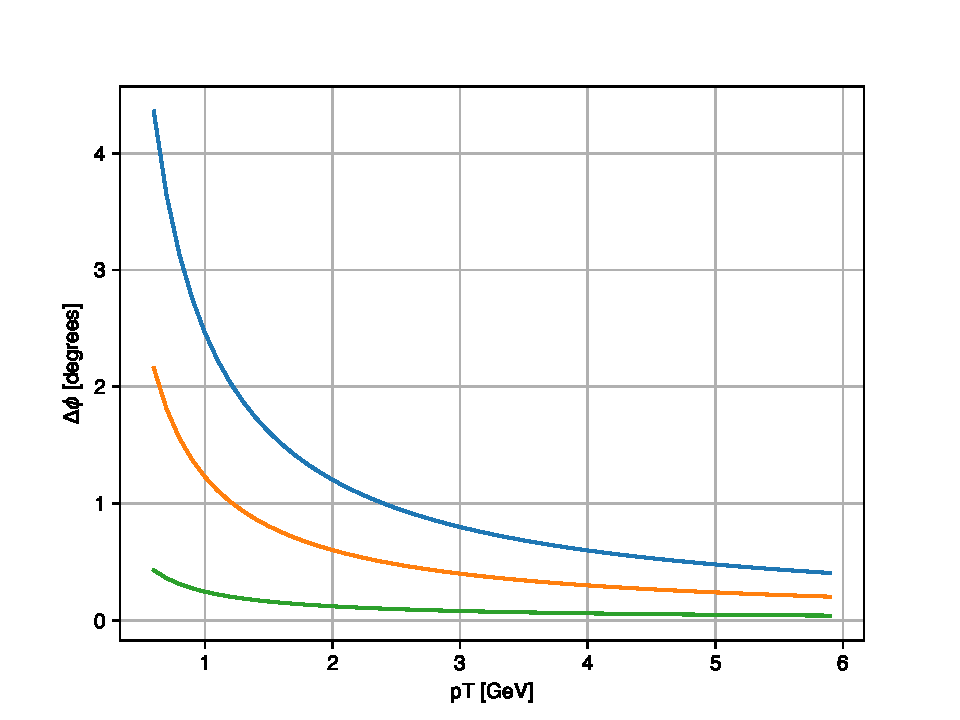
\includegraphics[width=0.7\linewidth]{images/phiDeviation.pdf}
  \caption{Phi deviation as a function of \pt of a particle track traversing from one barrel layer positioned at radius $r_1$ and a second positioned at radius $r_2$ for three cases. 
  Each case has $r_1 = 0.532$\,m however for the blue line, the $r_2$ is 100\,mm further out, for the orange line 50\,mm further out and for the green line 10\,mm further out.}
  \label{fig:phiDeviation}
\end{figure}

\begin{table}
  \centering
  \begin{tabular}{ccc}
    \toprule
    $r_1$ & $r_2$ & $\Delta \phi$ \\
    \midrule
    532 & 632 & 0.064 \\
    542 & 622 & 0.051 \\
    552 & 612 & 0.038 \\
    562 & 602 & 0.026 \\
    572 & 592 & 0.013 \\
    \bottomrule
  \end{tabular}
  \caption{Some numbers for the $\phi$ deviation for a particle with $\pt = 1$\,GeV.
  Distances are in mm, angles in radians.}
\end{table}



\begin{figure}
  \centering
  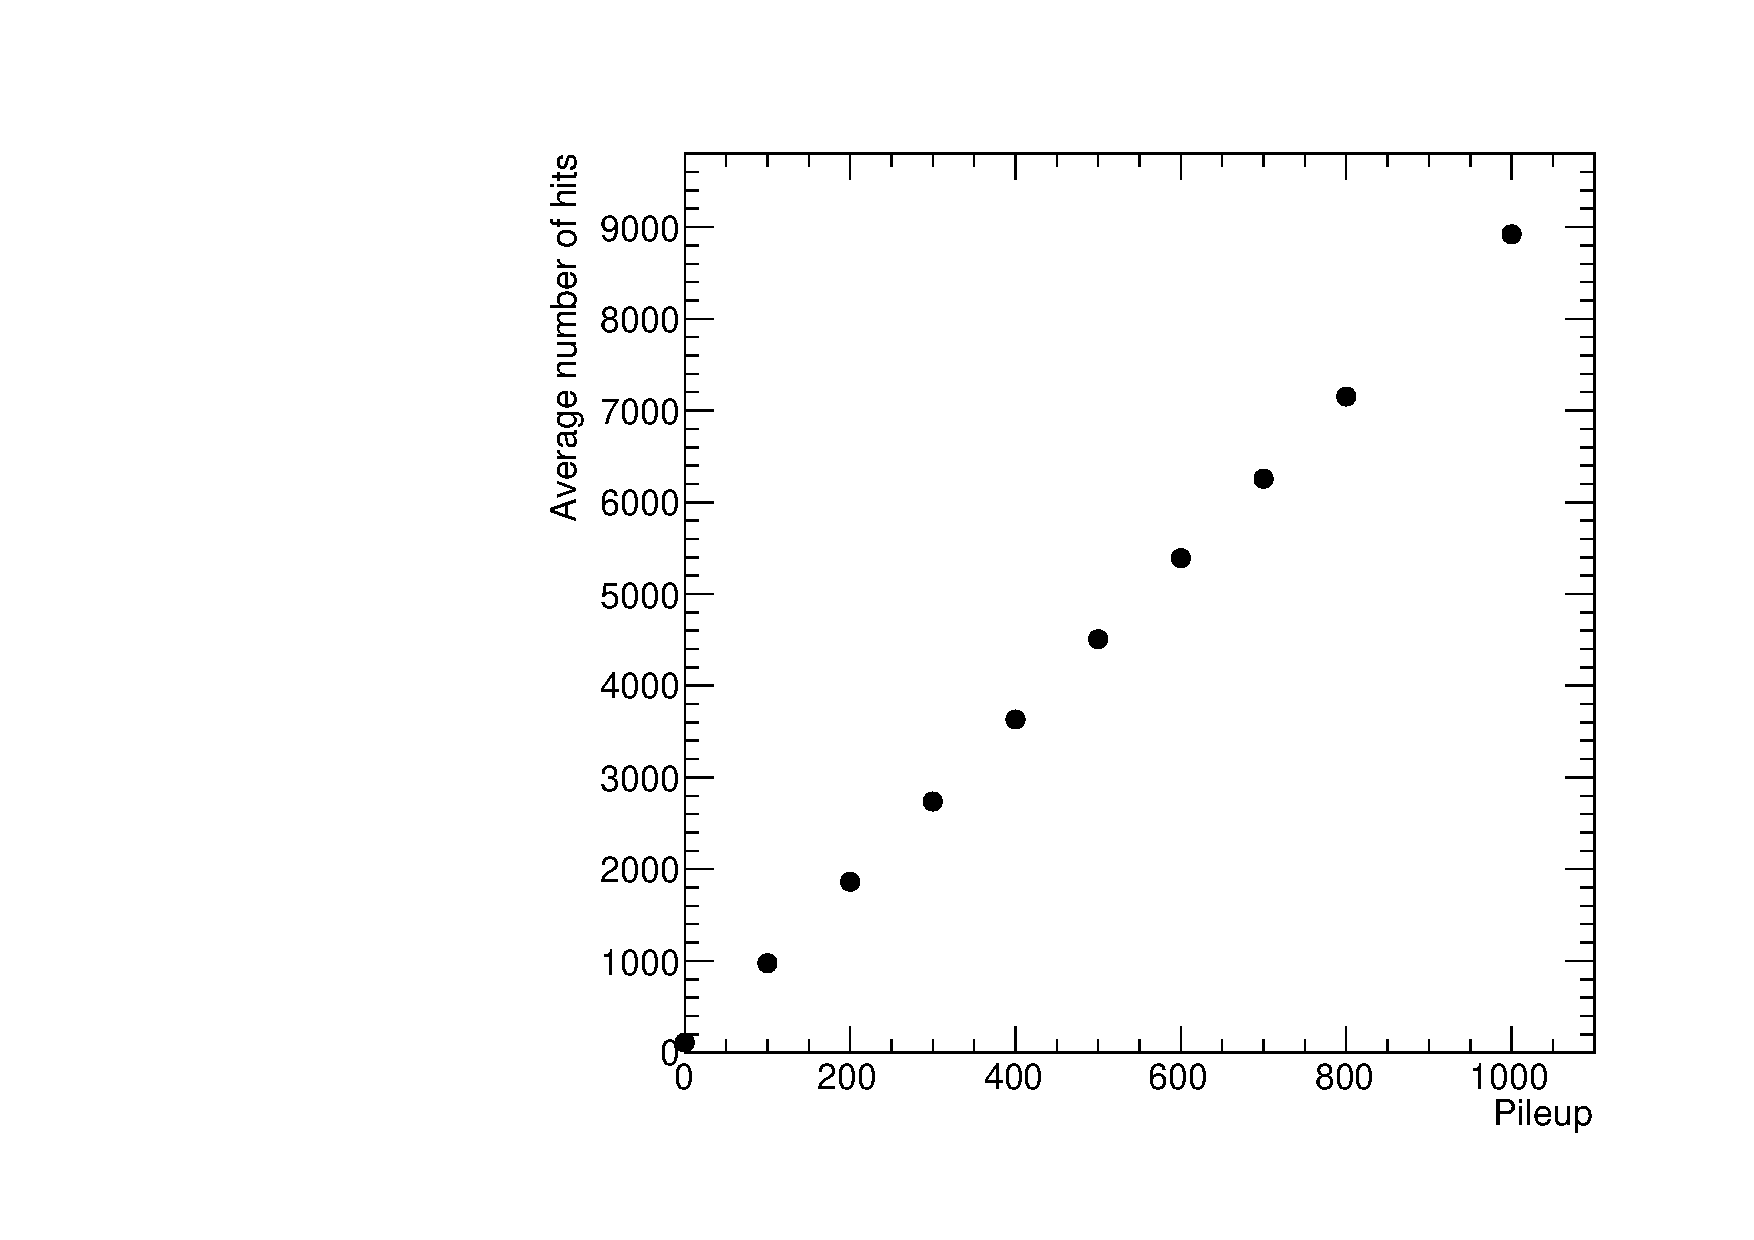
\includegraphics[width=0.5\linewidth,angle=-90]{images/pileup_hits}
  \caption{The number of hits in the outermost tracking layer (spacing 20mm) as a function of pileup.
  No transverse momentum cut is applied, other than that the hit must have reached the outermost layers.}
\end{figure}

\end{document}
